\documentclass[thesis.tex]{subfiles}
\def\x{\mathbf{x}}
\def\d{\mathbf{d}}
\def\w{\mathbf{w}}
\newcommand\TPR{\mathit{TPR}}
\newcommand\FPR{\mathit{FPR}}
\begin{document}

\chapter{Pedestrian detection}
\label{sec:od}
In this chapter we describe the pedestrian detection problem and how we apply our descriptor to solve it.

Object detection is the problem of locating specified objects in images. One application of this is pedestrian detection, which we have decided to focus on as it is simple and has extensive datasets. A common approach to object detection is to extract regions from the image, reducing the problem to binary classification of the presence of the specified object in each region. Using this approach, we are able to compute one descriptor for each region. We furthermore assume fixed size regions in scale-space, allowing us to directly compare our descriptors. The classification of pedestrians is done using a linear SVM.

The chapter is structured as follows...

\section{Support vector machine}

Suppose we have some training data split into positive and negative elements. In our case these are $n$-dimensional descriptors of regions with and without pedestrians. We wish to construct a binary classifier which accurately assigns a classification score denoting how confident we are that there is or isn't a pedestrian present. The approach of a linear support vector machine (SVM) is to place a $(n-1)$-dimensional hyperplane in descriptor space which separates the two classes. The hyperplane $(\w,b)$ is defined as the points $\x$ satisfying
%
\begin{align*}
\w \cdot \x - b = 0.
\end{align*}
%
If the data is linearly separable, we can search for the \emph{maximum-margin} hyperplane defined as having the largest possible distance to the nearest point of each class. This distance defines the margin. Formally, this can be written as the constrained optimization problem
%
\begin{align*}
\min_{\w,b} \frac12 \| \w \|^2 \qquad \text{subject to} \qquad y_i (\w \cdot \x_i - b) \geq 1,
\end{align*}
%
where $\x_i$ are training data points and $y_i \in \{-1,1\}$ their respective condition labels.

However, linear separation of the two classes is almost never feasible. Instead a \emph{soft-margin} SVM is used. The idea is to allow some of the data points to be placed on the wrong side of the margin. The total distance of misplaced points to the margin is minimized, in addition to maximizing the margin. This is done by introducing a \emph{cost} parameter $C$ which weights the importance of the misplacement minimization relative to the margin maximization. Formally, the soft-margin optimization problem is written as
%
\begin{align}
\label{eq:svmDefinition}
\min_{\w,\boldsymbol{\xi},b} \left\{ \frac12 \| \w \|^2 + C \sum_i \xi_i \right\} \qquad \text{subject to} \qquad \begin{aligned} y_i (\w \cdot \x_i - b) &\geq 1 - \xi_i, \\ \xi_i &\geq 0, \end{aligned}
\end{align}
%
where $\xi_i$ are slack variables allowing for misplaced points.

If there is a large skew in the number of elements in each class, the larger class will dominate the misplacement term, and we will be less likely to find a good separation. In order to correct this skew, the cost parameter $C$ can be defined for each of the two classes individually. The simplest approach is dividing $C$ by the number of elements in the respective classes.

When using the SVM for solving the pedestrian detection problem, we use the $L_2$-regularized $L_2$ loss support vector classifier from LIBLINEAR v. 1.94\footnote{\url{http://www.csie.ntu.edu.tw/~cjlin/liblinear/}} \cite{fan2008liblinear}. The naming of this SVM type means that the $L_2$-norm is used for computing both $\| \w \|$ and $\xi_i$, as in \Cref{eq:svmDefinition}.

\section{Performance measures}

Having described the method of using a SVM for binary classification, we are now able to define a performance measure for the pedestrian detection problem. Recall that the an SVM gives us the signed distances $\w \cdot \d - b$ between each descriptor $\d$ and the hyperplane dividing the two classes: positive for pedestrians and negative for non-pedestrians. Since the SVM is trained to find the best separation between the classes, we can use this distance as the classification score $s$. Following the binary classification method described in \Cref{sec:binaryClassificationMeasures}, we are able to compute both the PR- and ROC-curves and their AUCs. In other words we vary a threshold on the distance to the hyperplane to get the two measures of the performance of a descriptor.

The dataset we use (described in \Cref{sec:odDataset}) has a large skew in the amount of positives and negatives. This is because the only positives are the exact cut-outs of pedestrians, while negatives can be anything else.
Recall that the PR measure is preferred when there is a large skew towards one of the classes of a binary classification, as described in \Cref{sec:binaryClassificationMeasures}. We will therefore be using the PR measure as performance measure for our pedestrian detection parameter study as well as testing. \Citet{dalal2005histograms} use the log-log plot of the ROC-curve as performance measure, and hence we will show test results for this performance measure as well. In order for this measure to make sense, the actual plot is defined as the logarithm of $1-\text{Recall}$ versus the logarithm of $\FPR$.
%
\section{Dataset}
\label{sec:odDataset}
%
The dataset we use for training and testing our descriptor on the pedestrian detection application is called the \emph{INRIA Person Dataset}\footnote{\url{http://pascal.inrialpes.fr/data/human/}} (from now on called the INRIA dataset) created by \citet{dalal2005histograms}. The purpose of this dataset is to evaluate methods on more challenging images, compared to the earlier MIT Pedestrian dataset \cite{papageorgiou2000trainable}.

It consists of various real world images grouped into two subsets: images with pedestrians (positives) and images without pedestrians (negatives). From the positive images, cut-outs of pedestrians are extracted and rescaled to a fixed size, such that the pedestrian in each cut-out is 96 pixels in height from their feet to shoulders. We extract our own cut-outs from the negative images. The size of the cut-outs are $64 \times 128$ pixels with a 3 pixel border to avoid boundary condition effects. In case a pedestrian cut-out is smaller than the defined size after resizing, the borders are replicated to achieve the desired dimensions.
The positive set only contains images of somewhat upright persons that initially were at least 100 pixels in height. In order to improve the robustness of the dataset against reflected images, each positive cut-out has its horizontally flipped image included as well.

The dataset has been pre-split into training and test data in order to compare methods fairly. The training data has a total of 2416 positive and 1218 negative images, while the test data has a total of 1126 positives and 453 negatives.

\Cref{fig:inriaExampleImages} shows examples of positive \subref{fig:inriaPositives} and negative \subref{fig:inriaNegatives} images from the INRIA dataset. From the positive examples we clearly see the high variety of upright positions and surroundings in the dataset.

%\newgeometry{left=2cm,right=2cm,top=3cm,bottom=3cm}
\begin{figure}[p]
	\centering
	\begin{subfigure}[t]{\textwidth}
		\centerline{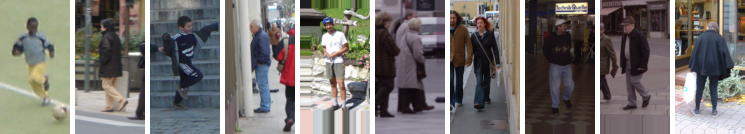
\includegraphics[width=1.2\textwidth]{img/inriaPositives.png}}
		\caption{Positives}
		\label{fig:inriaPositives}
		\vspace{2mm}
	\end{subfigure}
	\begin{subfigure}[t]{\textwidth}
		\centerline{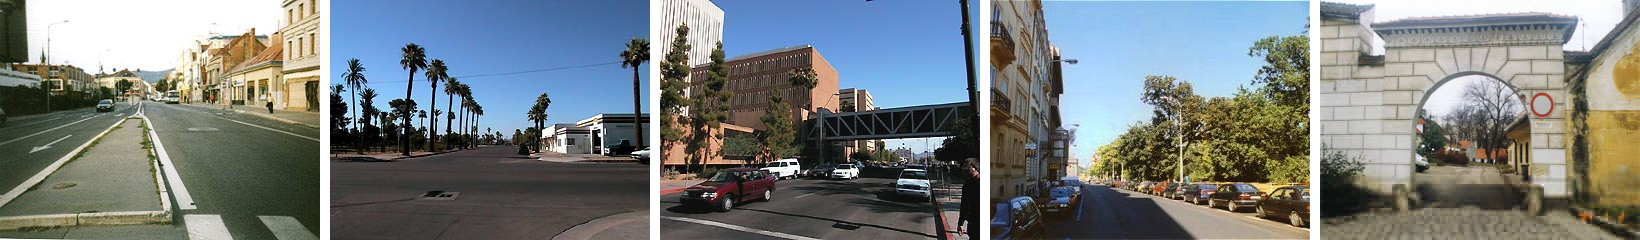
\includegraphics[width=1.2\textwidth]{img/inriaNegatives.png}}
		\caption{Negatives}
		\label{fig:inriaNegatives}
	\end{subfigure}
	\caption{Example INRIA images.}
	\label{fig:inriaExampleImages}
	%
	\vspace{1cm}
	%
	\centerline{
	\begin{subfigure}[t]{0.593\textwidth}
		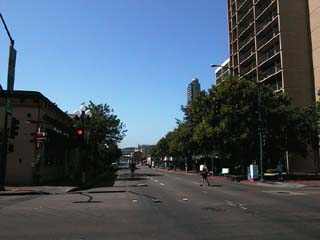
\includegraphics[width=\textwidth]{img/inriaManExample1.png}
	\end{subfigure}
	\begin{subfigure}[t]{0.593\textwidth}
		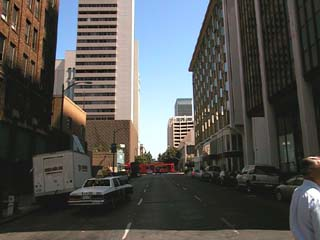
\includegraphics[width=\textwidth]{img/inriaManOccluded.png}
	\end{subfigure}
	}
	\caption{Examples of pedestrians in negative images.}
	\label{fig:inriaNegativePersons}
\end{figure}
%\restoregeometry

\subsection{Pitfalls and deficiencies}
We have found two minor problems with the INRIA dataset which could affect the results of using the dataset. The first problem is duplicate images. Amongst the negative training images we have found 10 pair-wise duplicates. This could bias the SVM since it effectively means that these images are weighted twice as high as the others. Given the small percentage of duplicates in the dataset the effect should however be close to nothing. We have also found a single duplicated image in the negative test set.

The second problem is the presence of people in some of the negatives.
\Cref{fig:inriaNegativePersons} show two examples of persons in the negative images of the INRIA dataset. The people are however either too small to fit correctly into the sliding window at any of the used scales or partially occluded by the image bounds to such an extent that we shouldn't be able to detect them anyway.

\section{Experimental setup}
\label{sec:inriaExperimentalSetup}
%
We have two experimental setups for evaluating descriptors on the INRIA dataset. The first is a validation setup for evaluating parameters during our parameter study using only the training data, and the second is a more complex test setup for evaluating the optimized or alternative descriptors on test data.

For our validation setup, we split the training data into six parts for the purpose of (leave-one-out) cross-validation. This is done by, for each split, training an SVM on five parts and testing on the other. The SVM is trained using all the given positive images and 40 random cut-outs from each negative image. The results are consolidated by computing the mean PR AUC across the six splits.

Our test setup is a modification of the one described by \citet{dalal2005histograms}. First, an SVM is trained using all positive training images and 40 random cut-outs from each negative training image. A sliding window is then run across these negative training images, and these windows are classified by the SVM in order to find false positives. In other words, we search the negative training images for examples that have not been learned by the SVM from the initial random cut-outs. These images are called \emph{hard negatives}. We pick a fixed number of hard negatives by finding the images with the $10^5$ largest classification scores (out of $2.2 \cdot 10^6$ total). These are the negative images our SVM is most uncertain about. We retrain an SVM with the added hard negatives, and test on the positive test images and sliding windows across negative test images.

Compared to \citet{dalal2005histograms}, we extract a lot more cut-outs (40 per image as opposed to 10) and add a lot more hard negatives ($10^5$ as opposed to just the positive classification scores). The old amounts of training examples were caused by hardware limitations of only having $1.7$ GB of RAM for SVM training. We also prefer using a fixed number of hard negatives in order to train the SVM on the same number of images for each descriptor.

\section{Example}
%
In this section we will show an example of our proposed GO descriptor calculated from a positive pedestrian image. Furthermore we illustrate the connection between the GO descriptor and the weights of a SVM classifier trained using the test setup in \Cref{sec:inriaExperimentalSetup}.
Finally we will show examples of the positive and negative images whose SVM classification we have most and least confidence in.

\Cref{fig:hogExample} shows a descriptor example from \citet{dalal2005histograms}, and \Cref{fig:inriaExample} shows the corresponding images reproduced for our GO descriptor. Since HOG has each histogram of gradients ``repeated'' by using block normalization, only the blocks centered at each pixel are illustrated. Our descriptor is illustrated for each cell of the descriptor. The average gradient images over the training data in \subref{fig:inriaPosTrainMeanM} are similar to one another, as they both are computed using central difference filters without smoothing. Likewise we clearly see the silhouette of a pedestrian in these average images.

The maximal positive and minimal negative SVM weights in \subref{fig:inriaExampleDescriptorSvmMax} and \subref{fig:inriaExampleDescriptorSvmMin} differ quite a lot since our descriptor has a much more dense grid. There are however some overall similarities such as large weights around the head and foot regions of the positive weights, at large weights inside the chest region of the negative SVM weights. In other words structure around the head and foot regions count towards a pedestrian detection and structure inside the chest region counts against a pedestrian detection.

Having described the SVM weights, we now look at the descriptors in \subref{fig:inriaExampleDescriptor} computed from the images in \subref{fig:inriaExampleCells}. The descriptors weighted by the positive and negative SVM weights are illustrated in \subref{fig:inriaExampleDescriptorSvm} and \subref{fig:inriaExampleDescriptorSvmNeg} respectively. Both HOG and our descriptor clearly visualize the pedestrian in \subref{fig:inriaExampleDescriptorSvm}. From \subref{fig:inriaExampleDescriptorSvmNeg} we see that vertical lines inside the pedestrian count against a pedestrian detection. The HOG example however weights these lines higher than our SVM, which for some reason weights the horizontal lines in the border high.

To get an idea of the types of images our trained SVM is best and worst at classifying, we find some of the pedestrian and non-pedestrian images with the highest and lowest classification scores. We call the pedestrian images with high classification scores true positives, as we are more likely to classify them correctly. Whether we do so of course depends on the exact threshold chosen. Similar statements can be said for false positives, true negatives, and false negatives. The images are shown in \Cref{fig:ownDescriptorExample}.

Generally the true positive images show pedestrians in standard up-right poses, with clothing clearly distinctive from the background, and having little to no occlusions. The false negatives are quite the opposite, and many have dim lighting with the person hard to make out. The true negative examples are all sky, with very little gradient structure. The false positives are quite varied; some have vertical lines at places a person could stand, but it is not obvious to see how they could be classified as pedestrians.

\todo{If time permits: Add examples of edge case classifications with their visualized descriptors?}
%
%\newgeometry{left=2cm,right=2cm,top=3cm,bottom=3cm}
\begin{figure}[tb]
	\centerline{
	\begin{subfigure}[t]{0.17\textwidth}
		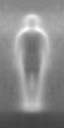
\includegraphics[width=\textwidth]{img/hogExample1.jpg}
		\caption{}
		\label{fig:hogExample1}
		\vspace{2mm}
	\end{subfigure}
	\begin{subfigure}[t]{0.17\textwidth}
		
\includegraphics[width=\textwidth]{img/hogExample2.png}
		\caption{}
		\label{fig:hogExample2}
		\vspace{2mm}
	\end{subfigure}
	\begin{subfigure}[t]{0.17\textwidth}
		
\includegraphics[width=\textwidth]{img/hogExample3.png}
		\caption{}
		\label{fig:hogExample3}
		\vspace{2mm}
	\end{subfigure}
	\begin{subfigure}[t]{0.17\textwidth}
		
\includegraphics[width=\textwidth]{img/hogExample4.jpg}
		\caption{}
		\label{fig:hogExample4}
		\vspace{2mm}
	\end{subfigure}
	\begin{subfigure}[t]{0.17\textwidth}
		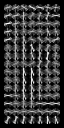
\includegraphics[width=\textwidth]{img/hogExample5.png}
		\caption{}
		\label{fig:hogExample5}
		\vspace{2mm}
	\end{subfigure}
	\begin{subfigure}[t]{0.17\textwidth}
		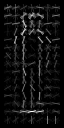
\includegraphics[width=\textwidth]{img/hogExample6.png}
		\caption{}
		\label{fig:hogExample6}
		\vspace{2mm}
	\end{subfigure}
	\begin{subfigure}[t]{0.17\textwidth}
		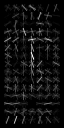
\includegraphics[width=\textwidth]{img/hogExample7.png}
		\caption{}
		\label{fig:hogExample7}
		\vspace{2mm}
	\end{subfigure}}
	\caption{Example of the HOG descriptor taken from \cite[Figure 6]{dalal2005histograms}. \subref{fig:hogExample1} shows the average gradient image over training data. \subref{fig:hogExample2} and \subref{fig:hogExample3} show the maximal positive and minimal negative SVM weights for each block centered at the pixels, respectively. \subref{fig:hogExample4} shows a test image. \subref{fig:hogExample5} shows its computed descriptor. \subref{fig:hogExample6} and \subref{fig:hogExample7} show the descriptor weighted by positive and negative SVM weights, respectively.}
	\label{fig:hogExample}
%	\stepcounter{figure}
	\vspace*{\floatsep}
	\setcounter{subfigure}{0}
	\centering
	\centerline{
	\begin{subfigure}[t]{0.1635\textwidth}
		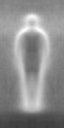
\includegraphics[width=\textwidth]{img/inriaPosTrainMeanM.png}
		\caption{}
		\label{fig:inriaPosTrainMeanM}
		\vspace{2mm}
	\end{subfigure}
	\begin{subfigure}[t]{0.17\textwidth}
		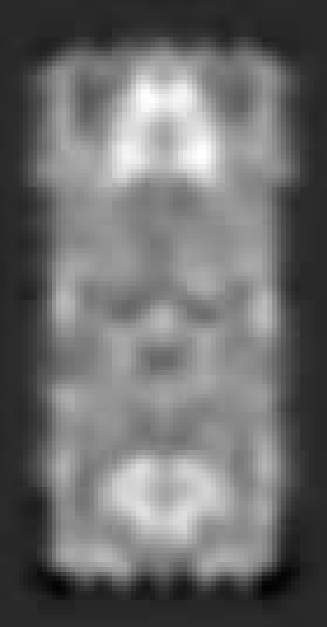
\includegraphics[width=\textwidth]{img/inriaExampleDescriptorSvmMax.pdf}
		\caption{}
		\label{fig:inriaExampleDescriptorSvmMax}
		\vspace{2mm}
	\end{subfigure}
	\begin{subfigure}[t]{0.17\textwidth}
		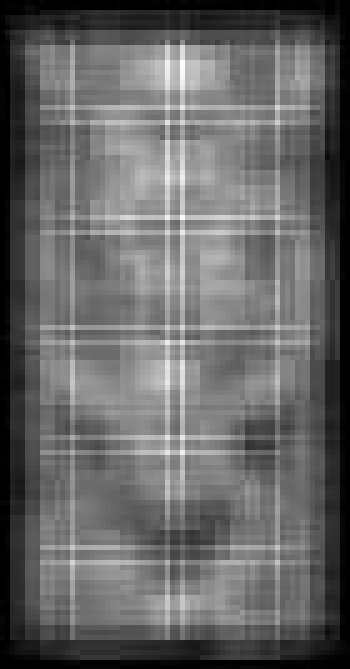
\includegraphics[width=\textwidth]{img/inriaExampleDescriptorSvmMin.pdf}
		\caption{}
		\label{fig:inriaExampleDescriptorSvmMin}
		\vspace{2mm}
	\end{subfigure}
	\begin{subfigure}[t]{0.17\textwidth}
		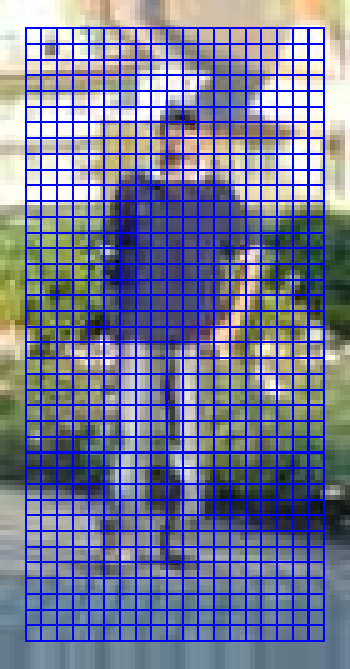
\includegraphics[width=\textwidth]{img/inriaExampleCells.pdf}
		\caption{}
		\label{fig:inriaExampleCells}
		\vspace{2mm}
	\end{subfigure}
	\begin{subfigure}[t]{0.17\textwidth}
		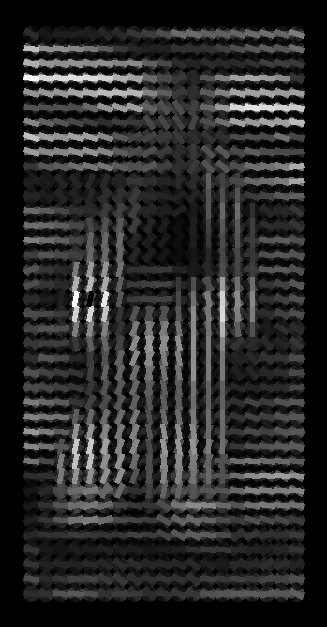
\includegraphics[width=\textwidth]{img/inriaExampleDescriptor.pdf}
		\caption{}
		\label{fig:inriaExampleDescriptor}
		\vspace{2mm}
	\end{subfigure}
	\begin{subfigure}[t]{0.17\textwidth}
		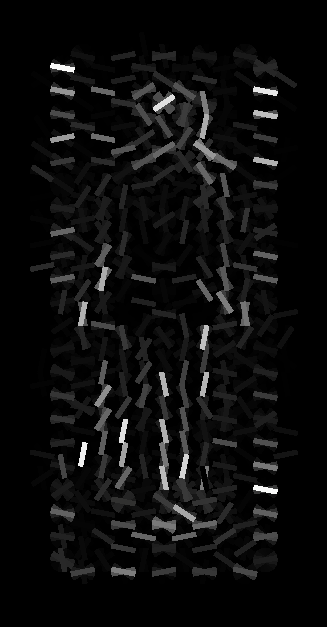
\includegraphics[width=\textwidth]{img/inriaExampleDescriptorSvm.pdf}
		\caption{}
		\label{fig:inriaExampleDescriptorSvm}
		\vspace{2mm}
	\end{subfigure}
	\begin{subfigure}[t]{0.17\textwidth}
		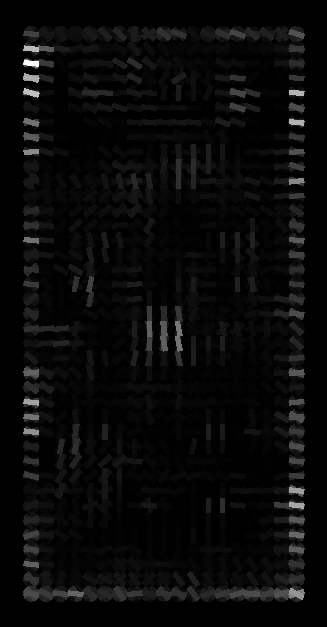
\includegraphics[width=\textwidth]{img/inriaExampleDescriptorSvmNeg.pdf}
		\caption{}
		\label{fig:inriaExampleDescriptorSvmNeg}
		\vspace{2mm}
	\end{subfigure}}
	\caption{Example of our GO descriptor following the same procedure as \Cref{fig:hogExample}. \subref{fig:inriaExampleDescriptorSvmMax} and \subref{fig:inriaExampleDescriptorSvmMin} are however shown for each cell instead of the HOG blocks, and upon \subref{fig:inriaExampleCells} we have illustrated out grid layout using the cell spacing $r$.}
	\label{fig:inriaExample}
\end{figure}
%\restoregeometry
%
%
\begin{figure}
	\begin{subfigure}[t]{\textwidth}
		\centerline{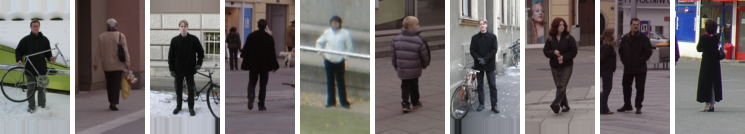
\includegraphics[width=1.2\textwidth]{img/objectDetectionTP.png}}
		\caption{True positives}
		\label{fig:objectDetectionTP}
		\vspace{2mm}
	\end{subfigure}
	\begin{subfigure}[t]{\textwidth}
		\centerline{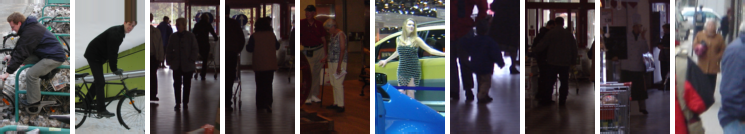
\includegraphics[width=1.2\textwidth]{img/objectDetectionFN.png}}
		\caption{False negatives}
		\label{fig:objectDetectionFN}
		\vspace{2mm}
	\end{subfigure}
	\begin{subfigure}[t]{\textwidth}
		\centerline{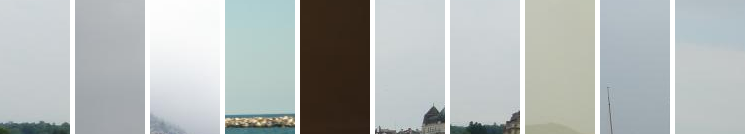
\includegraphics[width=1.2\textwidth]{img/objectDetectionTN.png}}
		\caption{True negatives}
		\label{fig:objectDetectionTN}
		\vspace{2mm}
	\end{subfigure}
	\begin{subfigure}[t]{\textwidth}
		\centerline{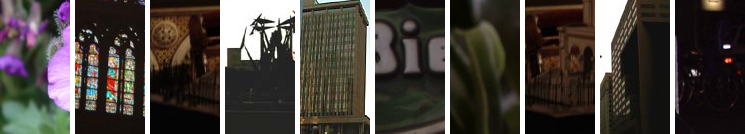
\includegraphics[width=1.2\textwidth]{img/objectDetectionFP.png}}
		\caption{False positives}
		\label{fig:objectDetectionFP}
	\end{subfigure}
	\caption{Example classifications of INRIA cut-outs.}
	\label{fig:ownDescriptorExample}
\end{figure}
%\restoregeometry

\section{Parameter study}
\label{sec:odParameterStudy}
%
We follow the same setup as the image correspondence parameter study.
%
\begin{figure}[p]
\centering
	\centerline{\begin{subfigure}[t]{0.593\textwidth}
		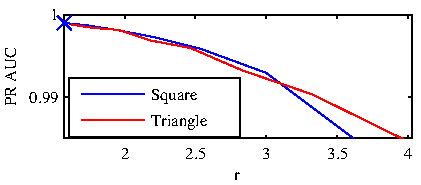
\includegraphics[width=\textwidth]{img/inriaParametersGo_cellSpacing.pdf}
		\caption{Cell spacing $r$}
		\label{fig:inriaParametersGo_cellSpacing}
	\end{subfigure}
	\begin{subfigure}[t]{0.593\textwidth}
		\centering
		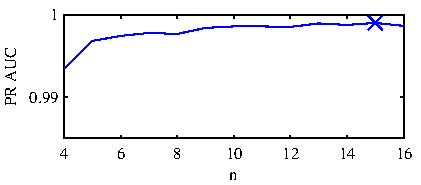
\includegraphics[width=\textwidth]{img/inriaParametersGo_binCount.pdf}
		\caption{Bin count $n$}
		\label{fig:inriaParametersGo_binCount}
	\end{subfigure}}
	\centerline{\begin{subfigure}[t]{0.593\textwidth}
		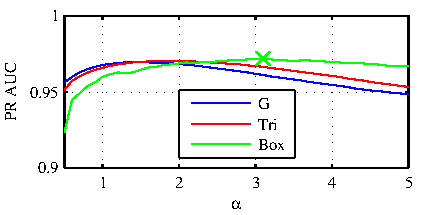
\includegraphics[width=\textwidth]{img/inriaParametersGo_cellSigmaAlt.pdf}
		\caption{Cell scale $\alpha$}
		\label{fig:inriaParametersGo_cellSigma}
		\vspace{2mm}
	\end{subfigure}
	\begin{subfigure}[t]{0.593\textwidth}
		\centering
		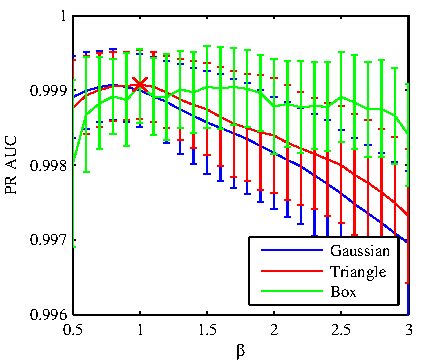
\includegraphics[width=\textwidth]{img/inriaParametersGo_binSigmaAlt.pdf}
		\caption{Bin scale $\beta$}
		\label{fig:inriaParametersGo_binSigma}
	\end{subfigure}}
	\centerline{\begin{subfigure}[t]{0.593\textwidth}
		\centering
		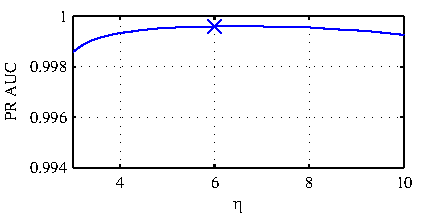
\includegraphics[width=\textwidth]{img/inriaParametersGo_normSigma.pdf}
		\caption{Normalization scale $\eta$}
		\label{fig:inriaParametersGo_normSigma}
		\vspace{2mm}
	\end{subfigure}
	\begin{subfigure}[t]{0.593\textwidth}
		\centering
		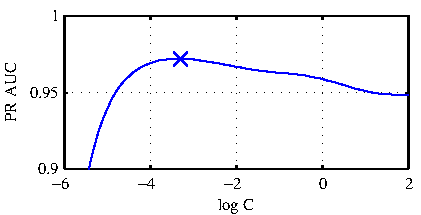
\includegraphics[width=\textwidth]{img/inriaParametersGo_logC.pdf}
		\caption{SVM weight $C$}
		\label{fig:inriaParametersGo_logC}
		\vspace{2mm}
	\end{subfigure}}
	\caption{Parameter study results for GO. We plot the cross-validation PR AUC for various parameter values, and mark the optimal values with a cross.}
	\label{fig:inriaParametersGoAuc}
	\vspace{1cm}
	\centerline{\begin{subfigure}[t]{0.593\textwidth}
		\centering
		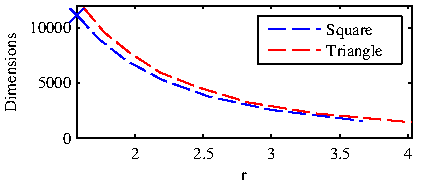
\includegraphics[width=\textwidth]{img/inriaParametersGo_cellSpacingDims.pdf}
		\caption{Cell spacing $r$}
		\label{fig:inriaParametersGo_cellSpacingDims}
	\end{subfigure}
	\begin{subfigure}[t]{0.593\textwidth}
		\centering
		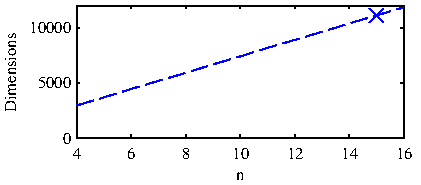
\includegraphics[width=\textwidth]{img/inriaParametersGo_binCountDims.pdf}
		\caption{Bin count $n$}
		\label{fig:inriaParametersGo_binCountDims}
		\vspace{2mm}
	\end{subfigure}}
	\caption{Dimensionality of our GO descriptor for various parameter values.}
	\label{fig:inriaParametersGoDims}
\end{figure}
%
\begin{figure}[p]
\centering
	\centerline{\begin{subfigure}[t]{0.593\textwidth}
		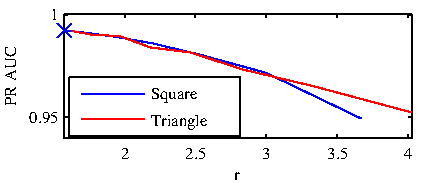
\includegraphics[width=\textwidth]{img/inriaParametersSi_cellSpacing.pdf}
		\caption{Cell spacing $r$}
		\label{fig:inriaParametersSi_cellSpacing}
	\end{subfigure}
	\begin{subfigure}[t]{0.593\textwidth}
		\centering
		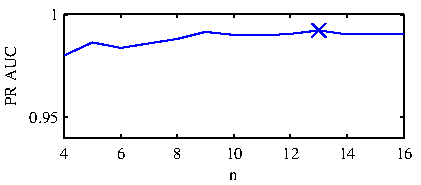
\includegraphics[width=\textwidth]{img/inriaParametersSi_binCount.pdf}
		\caption{Bin count $n$}
		\label{fig:inriaParametersSi_binCount}
	\end{subfigure}}
	\centerline{\begin{subfigure}[t]{0.593\textwidth}
		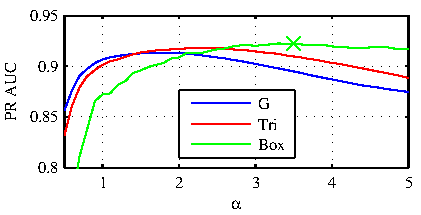
\includegraphics[width=\textwidth]{img/inriaParametersSi_cellSigmaAlt.pdf}
		\caption{Cell scale $\alpha$}
		\label{fig:inriaParametersSi_cellSigma}
		\vspace{2mm}
	\end{subfigure}
	\begin{subfigure}[t]{0.593\textwidth}
		\centering
		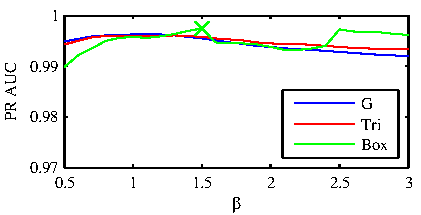
\includegraphics[width=\textwidth]{img/inriaParametersSi_binSigmaAlt.pdf}
		\caption{Bin scale $\beta$}
		\label{fig:inriaParametersSi_binSigma}
	\end{subfigure}}
	\centerline{\begin{subfigure}[t]{0.593\textwidth}
		\centering
		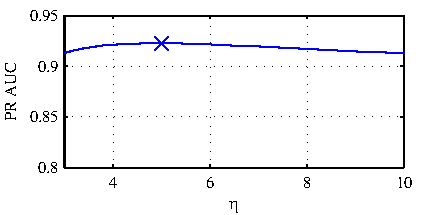
\includegraphics[width=\textwidth]{img/inriaParametersSi_normSigma.pdf}
		\caption{Normalization scale $\eta$}
		\label{fig:inriaParametersSi_normSigma}
		\vspace{2mm}
	\end{subfigure}
	\begin{subfigure}[t]{0.593\textwidth}
		\centering
		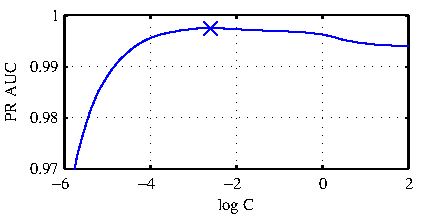
\includegraphics[width=\textwidth]{img/inriaParametersSi_logC.pdf}
		\caption{SVM weight $C$}
		\label{fig:inriaParametersSi_logC}
		\vspace{2mm}
	\end{subfigure}}
	\caption{Parameter study results for SI. We plot the cross-validation PR AUC for various parameter values, and mark the optimal values with a cross.}
	\label{fig:inriaParametersSiAuc}
	\vspace{1cm}
	\centerline{\begin{subfigure}[t]{0.593\textwidth}
		\centering
		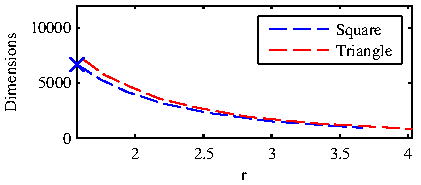
\includegraphics[width=\textwidth]{img/inriaParametersSi_cellSpacingDims.pdf}
		\caption{Cell spacing $r$}
		\label{fig:inriaParametersSi_cellSpacingDims}
	\end{subfigure}
	\begin{subfigure}[t]{0.593\textwidth}
		\centering
		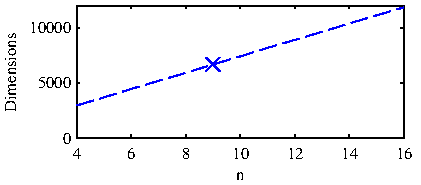
\includegraphics[width=\textwidth]{img/inriaParametersSi_binCountDims.pdf}
		\caption{Bin count $n$}
		\label{fig:inriaParametersSi_binCountDims}
		\vspace{2mm}
	\end{subfigure}}
	\caption{Dimensionality of our SI descriptor for various parameter values.}
	\label{fig:inriaParametersSiDims}
\end{figure}
% 
\begin{table}[tb]
\centering
\begin{tabular}{ l c c }
\toprule
{} & \multicolumn{2}{c}{Methods} \\
Variable & GO & SI \\ \midrule
Grid type & Square & Square \\
Cell spacing $r$ & $1.6$ & $1.6$ \\
Cell kernel & \textit{Box} & \textit{Box} \\
Cell scale $\alpha$ & $3.3$ & $3.5$ \\
Bin count $n$ & $15$ & $9$ \\
Bin kernel & \textit{Tri} & \textit{Box} \\
Bin scale $\beta$ & $1.0$ & $1.5$ \\
Normalization scale $\eta$ & $6.0$ & $5.0$ \\
\bottomrule
\end{tabular}
\caption{Parameter study from 6-fold cross validation for GO and SI}
\label{fig:INRIAparamC}
\end{table}
%
\begin{table}[tb]
\centering
\begin{tabular}{ l c c c c }
\toprule
{} & \multicolumn{4}{c}{Methods} \\
Variable & GO & SI & GO+SI & HOG \\ \midrule
$\log C$ & $1.3\cdot 10^{-3}$ & $2.5\cdot 10^{-3}$ & $1.6\cdot 10^{-3}$ & $1.3\cdot 10^{-3}$ \\
\bottomrule
\end{tabular}
\caption{Parameter study for optimal C parameter from 6-fold cross validation for GO, SI, GO+SI, and HOG}
\label{fig:INRIAparamC}
\end{table}
%
\section{Results}
%
Now that we have computed optimal parameters on the training data, we can evaluate the performance of the descriptors on test data. \Cref{fig:inriaTestResults} shows ROC- and PR-curves of the various descriptors. Both curves show the same ordering of descriptor performances, from best to worst: GO+SI, GO, compact GO, SI, HOG. The long straight line segments, which appear in both graphs, occur because there are many completely blank negative cut-outs that are all given the same classification score.

\Cref{fig:inriaHistogram} illustrates the distribution of classification scores for positive and negative images. This gives a more intuitive understanding of the performance of the descriptors. We see for instance that GO+SI achieves a much better separation of the two classes than HOG.
%
\begin{table}[tb]
\centering
\begin{tabular}{ l c c c c }
\toprule
Descriptor & Dimensions & PR AUC & ROC AUC & Recall at $10^{-4}$ FPR \\ \midrule
GO+SI & $17784$ & $0.9937$ & $0.999980$ & $0.982$ \\ 
GO & $11115$ & $0.9911$ & $0.999978$ & $0.982$ \\ 
Compact GO & $4185$ & $0.9874$ & $0.999962$ & $0.965$ \\ 
SI & $6669$ & $0.9668$ & $0.999803$ & $0.920$ \\ 
HOG & $4743$ & $0.9210$ & $0.998721$ & $0.854$ \\ 
\bottomrule
\end{tabular}
\caption{Results}
\label{tbl:inriaResults}
\end{table}
%
\begin{figure}[tb]
\centering
	\centerline{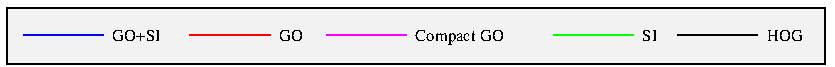
\includegraphics[width=1.2\textwidth]{img/inriaTestResultsLegend.pdf}}
	\centerline{\begin{subfigure}[t]{0.593\textwidth}
		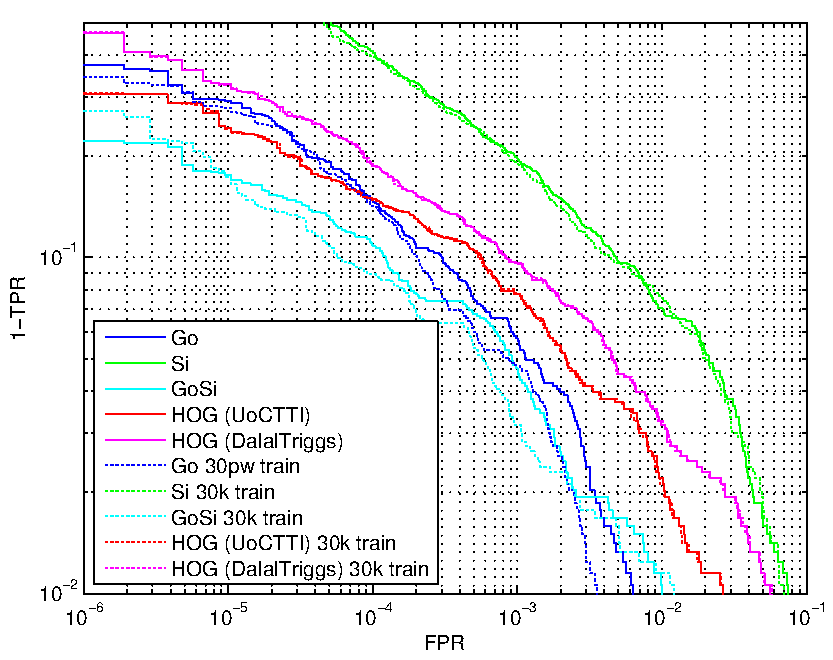
\includegraphics[width=\textwidth]{img/inriaTestResultsROC.pdf}
		\caption{Log-log ROC-curve}
		\label{fig:inriaTestResultsROC}
	\end{subfigure}
	\begin{subfigure}[t]{0.593\textwidth}
		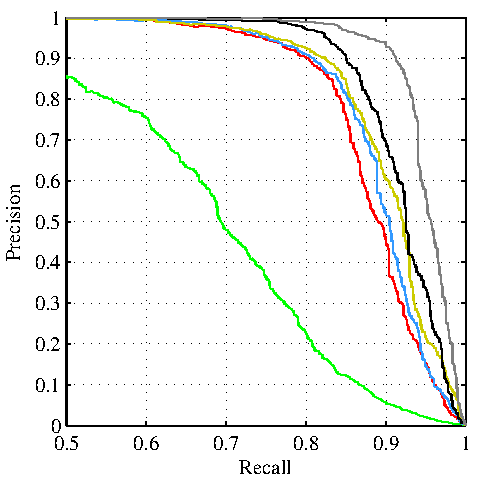
\includegraphics[width=\textwidth]{img/inriaTestResultsPR.pdf}
		\caption{PR-curve}
		\label{fig:inriaTestResultsPR}
	\end{subfigure}}
	\caption{INRIA test results.}
	\label{fig:inriaTestResults}
\end{figure}
%
\begin{figure}
	\centering
	\begin{subfigure}[t]{\textwidth}
		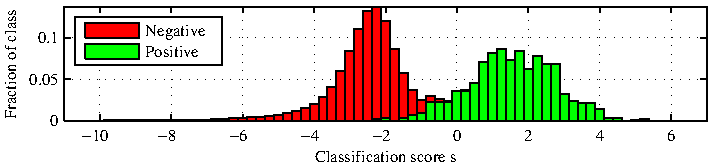
\includegraphics[width=\textwidth]{img/inriaHistogramGoSiFinal.pdf}
		\caption{GO+SI}
		\label{fig:inriaHistogramGoSiFinal}
	\end{subfigure}
	\begin{subfigure}[t]{\textwidth}
		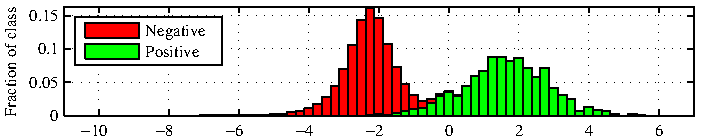
\includegraphics[width=\textwidth]{img/inriaHistogramGoFinal.pdf}
		\caption{GO}
		\label{fig:inriaHistogramGoFinal}
	\end{subfigure}
	\begin{subfigure}[t]{\textwidth}
		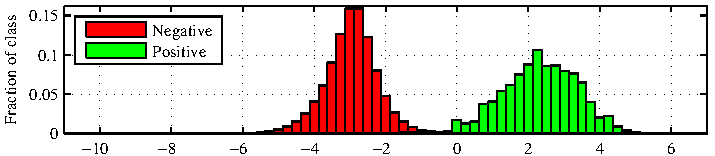
\includegraphics[width=\textwidth]{img/inriaHistogramGoChosenSmall.pdf}
		\caption{Compact GO}
		\label{fig:inriaHistogramGoChosenSmall}
	\end{subfigure}
	\begin{subfigure}[t]{\textwidth}
		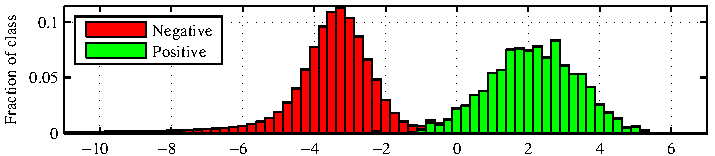
\includegraphics[width=\textwidth]{img/inriaHistogramSiFinal.pdf}
		\caption{SI}
		\label{fig:inriaHistogramSiFinal}
	\end{subfigure}
	\begin{subfigure}[t]{\textwidth}
		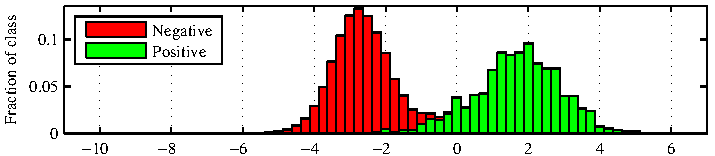
\includegraphics[width=\textwidth]{img/inriaHistogramHog.pdf}
		\caption{HOG}
		\label{fig:inriaHistogramHog}
	\end{subfigure}
	\caption{Histograms of classification scores on INRIA test data for various descriptors. The negative and positive results are individually normalized due to the large skew in amount of images.}
	\label{fig:inriaHistogram}
\end{figure}
%
\subbibliography

\end{document}
